\chapter{Pentesting}

\epigraph{\textit{''Si piensas que la tecnología puede solucionar tus problemas de seguridad, está claro que ni entiendes los problemas ni entiendes la tecnología''}}{--- Bruce Schneier}

Dentro de en la seguridad informática un test de intrusión, o \textit{pentesting}, como se conoce en inglés, evalúa los diferentes niveles de seguridad de un sistema informático red mediante la simulación en un entorno controlado de un ataque por parte de un usuario malicioso conocido comúnmente como hacker \cite{pentesting-kali}. El propósito de una prueba de penetración es determinar la viabilidad de un ataque y la cantidad de impacto que puede causar este mismo.

\section{Objetivos}

A día de hoy el pentesting es una de las técnicas más utilizadas para garantizar tanto la seguridad de la información como la propia seguridad informática de los sistemas de empresas u organizaciones. Es uno de los pilares básicos en las auditorías de seguridad informática, en las que empresas contratan a expertos en seguridad para evaluar la fortaleza de sus sistemas informáticos.

El pentesting no es un área con unas técnicas de actuación concretas. El pentesting usa una grandísima cantidad de técnicas, a las cuales se van añadiendo técnicas que van surgiendo, para determinar la seguridad de sistema informático y, en particular, conocer las debilidades que tiene el sistema informático.

Haciendo un símil con otras áreas completamente diferentes, un pentesting podría equivaler a una serie de pruebas prácticas que se realizan, por ejemplo, en controles de calidad para todo tipo de productos, en los cuales se ve que la mejor forma de probar el correcto funcionamiento de dichos productos consiste en someterlos a una serie de pruebas. Dichas pruebas están basadas en los entornos reales en los que se utilizan esos productos.

Por ejemplo: la mejor manera de probar la efectividad de un chaleco antibalas es realizando disparos sobre él para ver hasta qué punto los materiales como el Kevlar o de los tejidos que han sido compuestos para dicho chaleco son adecuados para parar una bala. De la misma manera, la mejor forma de probar si un sistema informático o una red compuesta de varios sistemas es segura, o mejor dicho, hasta qué punto es segura, es elaborar ciertas pruebas e intentar explotar vulnerabilidades que puedan surgir en estos sistemas. Todo ello con el objetivo final de sacar conclusiones y, en base a esas conclusiones, mejorar y fortificar ese sistema.

Aunque, de la misma manera que jamás se harían pruebas con el chaleco antibalas comprometiendo la integridad de ninguna persona física, tampoco se elabora un pentesting comprometiendo de manera real ningún sistema. El pentesting, al igual que las pruebas del chaleco, se elaboran ambas en un entorno controlado y limitado.

Teniendo en cuenta que la seguridad de los sistemas informáticos es vital para la continuidad del negocio de y el correcto desarrollo de las actividades de una empresa u organización, y siendo el pentesting una de las mejores herramientas para garantizar dicha seguridad, hace que este sea uno de los métodos más usados por todo tipo de empresas u organizaciones.


%------------------------------------------------------------------------------

\section{Partes}

Dentro de un pentesting se diferencian diferentes etapas cada una de las cuales tiene objetivos particulares y concretos. Aunque algunas de estas partes puedan tener sentido de manera independiente, en su conjunto permiten un completo análisis de un sistema informático del cual sacar conclusiones que permitan preservar la seguridad.

A continuación, se enumeran y definen las fases de un test de intrusión o pentesting, que ya se encuentran estandarizadas en el PTES (\textit{Penetration Testing Execution Standard}) \cite{ptes}:

\begin{figure}[H]
	\centering
	
\includegraphics[width=150px]{ptes}
	\caption{Logo de Penetration Testing Execution Standard}
	\label{fig:ptes}
\end{figure}

\begin{enumerate}
	\item \emph{Reglas del juego, alcance y términos del test de intrusión:} en esta fase se establece una serie de protocolos entre el realizador del pentesting (normalmente una auditoría de seguridad informática) y el auditado (normalmente una empresa u organización). En esta fase se establecen los objetivos a los que llegar, los límites a los que tendrán que adherirse los auditores.
	\item \emph{Recolección de información:} fase en la que se obtiene información del sistema para enfocar posteriormente analizarla.
	\item \emph{Análisis de las vulnerabilidades:} fase en la que mediante la información obtenida, se pasa a determinar las vulnerabilidades del sistema.
	\item \emph{Explotación de las vulnerabilidades:} tras determinar esas vulnerabilidades, se pasa a intentar explotarlas para visualizar su gravedad y el daño real que pueden causar.
	\item \emph{Postexplotación del sistema:} tras haber logrado explotar una vulnerabilidad, se intenta minar lo más posible el sistema, intentando lograr un efecto en cadena para ver, hasta qué punto, se puede dañar un sistema mediante una vulnerabilidad concreta.
	\item \emph{Generación de informes:} tras todos los pasos anteriores, se condensa todo el proceso elaborado y las conclusiones a las que se ha llegado en informes, de tal manera que a través de esos informes, se pueda actuar para corregir las vulnerabilidades y fortalecer el sistema.
\end{enumerate}

De todas esas fases, a continuación se profundizará en las más importantes.

\section{Recogida de información}

\textit{''La información es poder''}. Esa frase, atribuida a Francis Bacon (aunque se desconoce si realmente llegó a pronunciarla en algún momento), no podría ser más cierta actualmente. La informática no es más que la ciencia que trata la información, y la seguridad informática es un área que se encarga de protegerla. Por ello, a la hora de realizar un pentesting, resulta esencial obtener la mayor cantidad de información posible. El éxito de muchos de los ataques e intrusiones que sufren empresas y organizaciones se debe en gran parte a la gran cantidad de información que directa e indirectamente un atacante es capaz de obtener sobre sus sistemas \cite{inteco-gathering}.

Por ello, la fase de recogida de información o \textit{Information Gathering} resulta fundamental a la hora de realizar un test de intrusión. A mayor cantidad de información obtiene un atacante de un sistema mayor probabilidad de éxito tendrá al atacar.

La recogida de información, según desde qué punto se realiza, se puede separar en dos categorías: \textit{External Footprinting} e \textit{Internal Footprinting}. La primera hace referencia obtener información desde fuera del sistema y la segunda obtener información dentro del sistema.

\subsection{Internal Footprinting}

El Internal Footprinting engloba toda la recogida de información que se realiza una vez se tiene acceso, parcial o completo, al sistema o la red de la que se desea obtener la información. Este tipo de recogida de información no se realiza en la segunda fase de un pentesting, es decir, al comiendo del pentesting, sino que se realiza en la fase de post explotación del sistema, la quinta fase de un test de intrusión. Es lógico que, sin todavía haber explotado ninguna vulnerabilidad, y por ende no se haya accedido al sistema, no se pueda recoger información dentro de él.

\subsection{External Footprinting}

El External Footprinting engloba toda la recogida información, que al contrario que el Internal Footprinting, se realiza desde fuera del sistema. Este tipo de recogida información sí que se realiza en la segunda fase de un test de intrusión, y de hecho es el primer paso esencial a realizar. A través de diversas técnicas se busca obtener la mayor cantidad de información posible de una red o un sistema para, posteriormente, analizarla y encontrar vulnerabilidades.

Las técnicas de recogida de información englobadas dentro del External Footprinting se pueden dividir a su vez en dos subcategorías, en función del grado de agresividad de las mismas. 

\subsubsection{Active Footprinting}

Por un lado, está el descubrimiento activo, denominado Active Footprinting, que destaca por interactuar directamente con la infraestructura del sistema objetivo mediante consultas al DNS, análisis de las cabeceras HTTP, enumeración de puertos y sus servicios, etcétera \cite{pentesting-kali}. Seguidamente se explicarán brevemente en qué consisten algunas de estas técnicas, sin la intención de entrar en las herramientas de software concretas.

\paragraph{Escaneos DNS}

Una de las formas más comunes a la hora de obtener información consiste en obtener información de los servidores DNS. DNS (Domain Name Services) es un protocolo que permite la conversión entre direcciones de red numéricas, como son las IPs, y direcciones FQDN (Full Qualified Domain Name), que son direcciones del estilo \url{miweb.es}. De esta manera, DNS provee una capa de abstracción para hacer más sencillo las conexiones por parte de los usuarios y administradores a otros servicios.

La transformación de una dirección IP en un nombre de dominio se conoce como resolución DNS, y su proceso inverso (de nombre de dominio a IP) se conoce como resolución inversa. Este tipo de operaciones se da en los servidores DNS, de los cuales, mediante diferentes técnicas se puede extraer información relevante, hasta tal punto que se puede llegar a determinar ciertos aspectos de la topología de la red en la que se encuentra el sistema al que estamos intentando acceder.

\paragraph{Fingerprinting}

El Fingerprinting consiste en obtener información del propio sistema al que se intenta acceder. Datos como el sistema operativo y su versión o las aplicaciones que usa son esenciales a la hora de buscar vulnerabilidades que se puedan explotar en el sistema para lograr acceso a este, aunque no se limita solo a este tipo de datos. Obtener el servidor web que usa determinado dominio o el CMS (Content Management System) que usa dicho servidor web es fundamental a la hora de determinar vulnerabilidades concretas para dicho software. Existen herramientas tanto para obtener esta información como para relacionarla con bases de datos, previamente elaboradas, en las que se encuentran gran cantidad de vulnerabilidades que ya han sido detectadas.

\paragraph{SMTP}

Otra de las áreas mediante las que se puede obtener información es la relacionada con el protocolo SMTP. Con ello se puede obtener información de los dominios de correo electrónico usados hasta direcciones de correo electrónicas concretas, lo que permite centrarse en vulnerabilidades para dichos dominios. Esto deriva en que se pueda lograr suplantar la identidad de cierto usuario.

\subsubsection{Passive Footprinting}

Por otro lado se encuentra el descubrimiento pasivo, lógicamente denominado Passive Footprinting, que recurre a la consulta de la información previamente indexada por motores de búsqueda registros públicos, foros, etcétera, por lo que no interactúa directamente con el sistema a penetrar \cite{pentesting-kali}. 

\paragraph{Whois}

Whois es un protocolo TCP que permite obtener datos sobre el propietario de un nombre de dominio o una dirección IP. Entre los datos que se pueden obtener, se encuentran el correo electrónico, el nombre completo, la ciudad, el código postal o el número de teléfono del propietario. Estos datos son de fácil acceso, existiendo incluso herramientas web que te permiten obtener dicha información mediante el mencionado protocolo.

\paragraph{Hacking con buscadores}

Los buscadores como Google o Bing son utilizados por la gran mayoría para encontrar sitios web. Lo que no todo el mundo conoce es que se tratan de una poderosísima herramienta para obtener información adicional sobre uno o varios sitios web. La gran mayoría de buscadores disponen de parámetros avanzados de búsqueda que permiten buscar palabras concretas en las URLs, buscar por una determinada extensión o buscar dentro un sitio web concreto. De esta forma, si se sabe qué buscar, se puede obtener información sobre qué vulnerabilidades se pueden explotar en cierta página web.

Aparte de los buscadores tradicionales, también existen una serie de buscadores especializado en la búsqueda de dispositivos, enfocados al IoT, en los que se pueden buscar desde webcam hasta electrodomésticos, con la condición de que estén conectados a Internet. Estos buscadores, como Shodan\footnote{https://www.shodan.io/}, permite también filtrar búsquedas y realizar búsquedas avanzadas que permitan obtener información sobre otros sistemas que no sean directamente servidores web.

\paragraph{Social network engineering}

La ingeniería social, aunque no dispone de herramientas concretas, son técnicas para obtener información a partir de las redes sociales. En las redes sociales, muchas veces de manera inconsciente o sin comprender las consecuencias que puede acarrear, se comparte una gran cantidad de información personal que, bien analizada, puede ser determinante para elaborar un ataque concreto.

\section{Análisis de vulnerabilidades}

Una vez obtenida toda la información posible sobre el sistema, se pasa a la siguiente fase definida en el PTES, que consiste en analizar qué vulnerabilidades concretas se pueden explotar. La información recogida se usa para obtener como resultado final un listado de vulnerabilidades que se pueden llegar a explotar en el sistema. Esta fase de análisis pasa por tres periodos.

\subsection{Pruebas}

En el primer periodo se realiza una serie de pruebas basándose en la información que disponemos del sistema, que previamente hemos obtenido. La información que nos den estas pruebas es importante, cuanto mayor número de pruebas se realicen mediante el mayor número de herramientas y técnicas posible los resultados mejorarán. Estas pruebas se engloban en pruebas pasivas o activas.

\subsubsection{Activas}

Las pruebas activas requieren interactuar directamente con el componente a auditar. Tienen una estrecha relación con el Active Footprinting, ya que se basan en la información obtenida de esa manera. Dentro de éstas se incluyen las siguientes categorías:

\begin{itemize}
	\item \emph{Automatizadas:} mediante diversas herramientas de software se interactúa con el sistema, enviando peticiones, escaneando los servicios, etc.
	\item \emph{Conexión manual:} para evitar falsos positivos que puedan dar las pruebas automatizadas, se llevan a cabo pruebas manuales, que realizan los mismos pasos que las automáticas pero sin el uso de dichas herramientas de análisis de vulnerabilidades.
	\item \emph{Ofuscadas:} con el objetivo de evitar la detección o el bloqueo por parte de sistemas IDS (Intrusión Detection System), IPS (Intrusion Prevention System) o WAF (Web Application Firewall), se realizan pruebas que se comportan de manera diferenciada con las pruebas tradicionales, alargando tiempos de espera entre peticiones, modificando ciertos aspectos de las peticiones o alternando entre objetivos.
\end{itemize}

\subsubsection{Pasivas}

La pruebas pasivas consisten en analizar la información obtenida mediante Passive Footprinting. Analizar dicha información puede permitirnos suponer la existencia de cierta vulnerabilidad en el sistema. A diferencia de las pruebas activas, estas contienen un mayor componente subjetivo y abstracto.

\subsection{Validación}

Una vez elaboradas una serie de pruebas necesitamos correlar la información que nos ha dado esa serie de pruebas. En esta paso, el objetivo es enmarcar la vulnerabilidad encontrada en un apartado técnico, clasificándola en una serie de categorías e indentificándolas de una manera concreta. Esta clasificación se puede realizar a varios niveles.
El mas concreto consiste en identificarlas mediante, valga la redundancia, identificadores concretos como el \emph{CVE}\footnote{https://cve.mitre.org/} (Common Vulnerabilities and Exposures). También se puede hacer a un nivel más global, mediante las categorias marcadas en diversas normas, como pueden ser el \emph{NIST SP 800-53}\footnote{https://nvd.nist.gov/800-53} o la \textit{Guía OWASP}\footnote{https://www.owasp.org/}.
	
\subsection{Investigación}

Tras la identificación de una (o más) vulnerabilidad, y haberla categorizado correctamente, es necesario evaluar la gravedad de dicha vulnerabilidad. Para ello se procede a realizar una investigación sobre dicha vulnerabilidad. Esta investigación puede ser privada, elaborando pruebas a nivel interno, como ataques de fuerza bruta o configurar replicas del entorno mediante el uso de máquinas virtuales (VM) para emular el entorno real y hacer pruebas con ello.

\section[Explotación de vulnerabilidades]{Explotación de vulnerabilidades: Ataques de penetración}

Si en las dos secciones anteriores se ha explicado la recogida y el análisis de la información, respectivamente. Esas dos fases tienen como objetivo explotar una serie de vulnerabilidades. Esa es la esencia del pentesting, penetrar en un sistema mediante la explotación de dichas vulnerabilidades, realizando una serie de ataques a estos. Dependiendo del tipo de ataque, al vulnerabilidad que se explota o el objetivo del ataque, se pueden clasificar en prácticamente una infinidad de categorías. En los siguientes puntos se explican algunas de ellas, consideradas las más importantes.

\subsection{Ataques de contraseñas}
La contraseñas son un mecanismo de sobra conocido, que se remonta a mucho antes de la invención de la informática e incluso son anteriores a la propia formalización de la lógica que cimienta todo el desarrollo de la informática y la electrónica digital. Si desde la antigüedad se llevan usando las contraseñas para limitar el acceso solo a ciertas personas a ciertos sitios, en la actualidad se usan para limitar el acceso por parte de cierto usuario a cierto sistema o servicio informático. A día de hoy son, aun con el auge de métodos biométricos, la herramienta de control de acceso más usada.

Partiendo de esa base, los ataques de contraseñas son cualquier técnica o mecanismo orientados a descifrar o romper las contraseñas usadas para proteger esos sistemas. Cabe destacar que todo mecanismo de autenticación por contraseñas se basa en la comparación de \emph{hashes} y no en la comparación de contraseñas, dando autorización solo cuando el hash de la contraseña introducida coincide con el almacenado previamente, que ha sido generado con anterioridad mediante la contraseña elegida para la protección de ese sistema.

Un \emph{hash} no es más que una cadena alfanumérica de longitud fija, la cual se genera en base a una \emph{función hash}. La esencia de esas funciones radica en que generar un hash es sencillo y poco costoso, pero obtener la cadena original (es decir, la contraseña) mediante el hash es extremadamente complicado, aunque dicha complejidad depende del algoritmo usado. Ejemplos de dichos algoritmos son SHA-1 o MD5.

\subsubsection{Fuerza bruta}

Lo ataques de contraseñas se pueden elaborar de varias maneras. El método mas básico es el de fuerza bruta, que como su nombre indica, consiste en probar todas las combinaciones posibles de contraseñas. Esto puede ser especialmente costoso a nivel computacional. En las Tablas \ref{table:contrasenas} y \ref{table:contrasenas-explotar} se puede ver la cantidad de contraseñas posibles para diferentes casos, ademas de cuanto tiempo costaría romper cada una en el peor de los casos.

\begin{table}[H]
	\centering
	\begin{tabular}{ |l|l|r| } 
		\hline
		\multicolumn{1}{|c|}{Contraseña} & 
		\multicolumn{2}{|c|}{Posibilidades} \\
		\hline
		Numérica de 4 caracteres 				& $ 10^4 $						& 10000 					\\
		Numérica de 6 caracteres 				& $ 10^6 $ 						& 1000000				 	\\
		Numérica de 8 caracteres 				& $ 10^8 $ 						& 100000000 			 	\\
		Numérica de 4 a 8 caracteres 			& $ \sum_{n=4}^{8} 10^{n} $ 	& 111110000 				\\
		\hline
		Alfanumérica de 4 caracteres 			& $ 27^4  $ 					& 531441  				 	\\
		Alfanumérica de 6 caracteres 			& $ 27^6 $ 						& 387420489  				\\
		Alfanumérica de 8 caracteres			& $ 27^8 $ 						& 282429536481 			 	\\
		Alfanumérica entre 4 y 8 caracteres		& $ \sum_{n=4}^{8} 27^{n} $		& 293292190521 				\\
		Alfanumérica entre 8 y 16 caracteres 	& $ \sum_{n=8}^{16} 27^{n} $	& 82834383195202897568241	\\
		\hline
	\end{tabular}
	\caption{Número de diferentes combinaciones de contraseñas contraseñas posibles para diferentes conjuntos}
	\label{table:contrasenas}
\end{table}

\begin{table}[H]
	\centering
	\begin{tabular}{ |l|r|r| } 
		\hline
		\multicolumn{1}{|c|}{Contraseña} & 
		\multicolumn{1}{|c|}{Tiempo CPU\tablefootnote{Teniendo en cuenta que se pueden probar una media de 1000 contraseñas por segundo mediante un núcleo de una CPU potente \cite{passhack-cpu}}} & 
		\multicolumn{1}{|c|}{Tiempo GPU\tablefootnote{Teniendo en cuenta que se pueden probar una media de 7000 contraseñas por segundo mediante un una GPU Nvidia GTX 1080 \cite{passhack-gpu}}} \\
		\hline		
		Numérica de 4 caracteres 				& 10 segundos			& 1,43 segundos 		\\
		Numérica de 6 caracteres 				& 16,66 minutos			& 2.381 minutos 		\\
		Numérica de 8 caracteres 				& 27,78 horas			& 3.97 horas 			\\
		Numérica de 4 a 8 caracteres 			& 30,86 horas 			& 4,40 horas 			\\
		\hline
		Alfanumérica de 4 caracteres 			& 8,85 minutos 			& 75,92 segundos		\\
		Alfanumérica de 6 caracteres 			& 4,48 días				& 15.37 horas			\\
		Alfanumérica de 8 caracteres			& \textsl{107,46 meses} & \textsl{15,36 meses}	\\
		Alfanumérica entre 4 y 8 caracteres		& \textsl{803540 años} 	& \textsl{114791 años}	\\
		Alfanumérica entre 8 y 16 caracteres 	& 2.62 billones de años \tablefootnote{1 Billón de años = 1.000.000 de millones de años} &  375237,29 millones de años \\
		\hline
	\end{tabular}
	\caption{Coste computacional de diferentes ataques de fuerza bruta para diferentes conjuntos}
	\label{table:contrasenas-explotar}
\end{table}

Se puede observar que, al menos mediante fuerza bruta y con un único ordenador estándar los ataques de fuerza bruta son prácticamente inútiles cuando la contraseña resulta ser mínimamente larga o compleja. Aun así, mediante supercomputadores y optimizaciones se pueden reducir tiempos, pero siguen siendo soluciones poco eficientes. 

\subsubsection{Por diccionario}

Por otra parte existen los denominado ataques de diccionario. En informática un diccionario consiste en una lista de palabras cualquiera, tengan sentido o no. Los ataques por diccionario simplemente prueban todas las opciones de un diccionario. Estos diccionarios se pueden obtener de diversas fuentes, o se pueden generar en base a palabra que guarden relación con el objetivo a atacar. De esta manera solo se prueban las combinaciones de caracteres que tengan mas posibilidades de aparecer, reduciendo drásticamente el tiempo que dura el ataque.

\subsection{Exploits}

El concepto de \emph{exploit} es sumamente sencillo. Un exploit no es más que una pequeña aplicación escrita con el objetivo de aprovecharse de una vulnerabilidad conocida en un software. La palabra proviene del inglés, que significa literalmente aprovechar o explotar. Los exploits son la parte más importante a la hora de explotar vulnerabilidades.

Ligando íntimamente al concepto de exploit existe el concepto de \emph{payload}. un payload no es más que una parte de código que el exploit se encarga de ejecutar en la máquina que tiene como víctima, normalmente con el objetivo de realizar algún tipo de acción maliciosa. Acciones como implementar una shell, añadir un usuario al sistema, borrar ciertos archivos o prácticamente lo que al ataque antes se le pueda ocurrir.

Según como sea los payloads se pueden clasificar en tres tipos:
\begin{enumerate}
	\item Los \emph{singles}: simplemente son código que se encarga de ejecutar una tarea concreta.
	\item Los \emph{stagers}: son payloads encargados de crear la conexión entre el atacante y la víctima normalmente este tipo de payloads preparan el terreno para los payloads de tipo \textit{staged}.
	\item Los \emph{staged}: son payload con funcionalidades más complejas, que son introducidos por los stagers en las máquinas a atacar.
\end{enumerate}

Sin querer profundizar demasiado en un campo al que se le podría bien dedicar libros enteros, mencionar que existen una gran cantidad de exploits ya detectados, es más, existen grandes bases de datos de exploits para ser usados por parte de la comunidad de la seguridad informática. Además existen también gran cantidad herramientas que permiten descargar, actualizar, gestionar, e inyectar estos exploits.

\subsection{Ataques a redes}

Los ataques a redes son un tipo de ataques que tienen como objetivo penetrar en una red informática para poder obtener información del tráfico interno de ésta. Una red informática puede tener diferentes topologías y dependiendo de ésta las características del ataque cambiarán drásticamente. El escenario varía de atacar una red PAN (\textit{Personal Area Network}) a atacar una red LAN (\textit{Local Area Network}) o WAN (\textit{Wide Area Network}). También dependiendo de si la red es inalámbrica o no el ataque se podrá elaborar de una u otra manera.

Los ataques se suelen enfocar a las diferentes capas del modelo de red, y más concretamente a los protocolos específicos que lo componen. El modelo de red extendido actualmente es el modelo \textbf{TCP/IP} que toma su nombre de los dos protocolos mas importantes de éste. Los diferentes protocolos usados en cada capa del modelo TCP/IP se pueden observar en la Figura \ref{fig:tcpip}.

\begin{figure}[H]
	\centering
	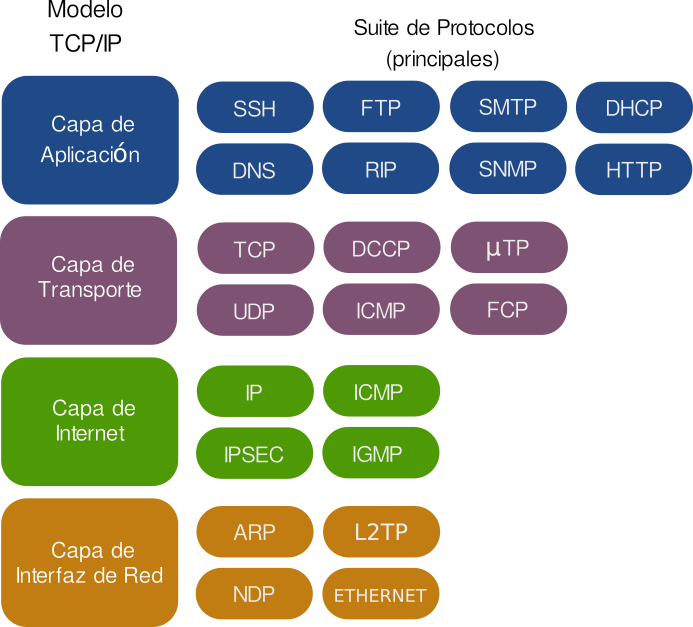
\includegraphics[width=0.8\textwidth]{tcpip}
	\caption{Principales protocolos usados en las 4 capas de TCP/IP}
	\label{fig:tcpip}
\end{figure}

Existen, independientemente del modelo, diferentes términos que destacan en los ataques a redes, como son el \textit{sniffing}, el \textit{spoofing} o el \textit{hijacking}.

\subsubsection{Sniffing}

El \emph{sniffing} es una técnica que consiste en capturar los paquetes o tramas que pasan por cierta interfaz \cite{ataque-en-redes-ip}. Por defecto un sistema rechaza el tráfico que no esta dirigido a én. En cambio, si un sistema actúa en modo promiscuo, aceptara todos los paquetes que le lleguen por la red. El sniffing es la técnica que obtiene todos esos paquetes. Para hacerlo, se hacen uso de herramientas llamadas \textit{sniffers}, que permiten capturar estos paquetes y analizar su información capa por capa.

\subsubsection{Spoofing}

\emph{Spoofing} es un concepto que consiste en suplantar la identidad \cite{ataque-en-redes-ip}. Existen numerosas técnicas de suplantación como por ejemplo \textit{MAC Spoofing}, donde se suplanta la dirección física de un dispositivo. También existen otras como \textit{ARP Spoofing}, \textit{DNS Spoofing} o \textit{Web Spoofing}. Consisten básicamente en falsear cierta información para hacernos pasar por otro usuario, otro nodo o otra aplicación en la red.

\subsubsection{Hijacking}

Se conoce como \emph{hijacking} a toda técnica en la que se obtiene el control de un elemento de una red, de tal manera que se pueda modificar la información que pasa por él \cite{ataque-en-redes-ip}. Existen, al igual que con el spoofing, numerosas técnicas que hacen uso del concepto, como por ejemplo Session Hijacking o Browser Hijacking. De este tipo de técnicas surgen los ataques MITM (\textit{Man In The Middle}), que como su nombre indica, consisten en interferir en la comunicación entre dos nodos para tanto suplantar la identidad del usuario como para recibir información que se supone que solo debería recibirla directamente el usuario.